% Created 2022-06-08 Wed 09:26
% Intended LaTeX compiler: xelatex
\documentclass[letterpaper]{article}
\usepackage{graphicx}
\usepackage{longtable}
\usepackage{wrapfig}
\usepackage{rotating}
\usepackage[normalem]{ulem}
\usepackage{amsmath}
\usepackage{amssymb}
\usepackage{capt-of}
\usepackage{hyperref}
\usepackage[margin=1in]{geometry}
\setlength{\parindent}{0pt}
\usepackage[margin=1in]{geometry}
\usepackage{fontspec}
\usepackage{svg}
\usepackage{tikz}
\usepackage{cancel}
\usepackage{pgfplots}
\usepackage{indentfirst}
\setmainfont[ItalicFont = HelveticaNeue-Italic, BoldFont = HelveticaNeue-Bold, BoldItalicFont = HelveticaNeue-BoldItalic]{HelveticaNeue}
\newfontfamily\NHLight[ItalicFont = HelveticaNeue-LightItalic, BoldFont       = HelveticaNeue-UltraLight, BoldItalicFont = HelveticaNeue-UltraLightItalic]{HelveticaNeue-Light}
\newcommand\textrmlf[1]{{\NHLight#1}}
\newcommand\textitlf[1]{{\NHLight\itshape#1}}
\let\textbflf\textrm
\newcommand\textulf[1]{{\NHLight\bfseries#1}}
\newcommand\textuitlf[1]{{\NHLight\bfseries\itshape#1}}
\usepackage{fancyhdr}
\usepackage{csquotes}
\pagestyle{fancy}
\usepackage{titlesec}
\usepackage{titling}
\makeatletter
\lhead{\textbf{\@title}}
\makeatother
\rhead{\textrmlf{Written} \today}
\lfoot{\theauthor\ \textbullet \ \textbf{2021-2022}}
\cfoot{}
\rfoot{\textrmlf{Page} \thepage}
\renewcommand{\tableofcontents}{}
\titleformat{\section} {\Large} {\textrmlf{\thesection} {|}} {0.3em} {\textbf}
\titleformat{\subsection} {\large} {\textrmlf{\thesubsection} {|}} {0.2em} {\textbf}
\titleformat{\subsubsection} {\large} {\textrmlf{\thesubsubsection} {|}} {0.1em} {\textbf}
\setlength{\parskip}{0.45em}
\renewcommand\maketitle{}
\author{Houjun Liu}
\date{\today}
\title{QIC Module 2: Changing Cubits}
\hypersetup{
 pdfauthor={Houjun Liu},
 pdftitle={QIC Module 2: Changing Cubits},
 pdfkeywords={},
 pdfsubject={},
 pdfcreator={Emacs 28.0.91 (Org mode 9.5.2)}, 
 pdflang={English}}
\begin{document}

\maketitle
\tableofcontents


\section{To Do}
\label{sec:org008742d}
\begin{itemize}
\item Read chapters
\item Watch videos
\end{itemize}

\section{Core Concepts}
\label{sec:orgf66603f}
\begin{itemize}
\item Solving the Shrödinger equation
\item We still look at a cubit at a time, but time will now pass: which impacts
the state of the cubit
\item We will learn about evolving a cubit, and gates, etc.
\end{itemize}

\section{Introduction}
\label{sec:org316b907}

\begin{equation}
   |ud \big> = u \big> \otimes |d\big> = \begin{pmatrix}
1 \\ 0 \end{pmatrix} \otimes \begin{pmatrix}
0 \\ 1 \end{pmatrix} = \begin{pmatrix}
0 \\ 1\\0\\0 \end{pmatrix}
\end{equation}

Instead of thinking about it as \emph{physics}, we will think it about computation.

We propagate \emph{square roots} of probabilities because time is not real, but is imaginary. The location of something is simply differently likely in various places.

Every \emph{property} in the quantum work as a cubit.

Change in perspective! Instead of simulating the behavior of cubits with bits, we can simulate them with OTHER CUBITS! So, our tools are now manipulating groups of cubits to simulate other, more complicated groups of cubits.

\section{Shrödinger's Equations}
\label{sec:org1d800a0}
\begin{equation}
   |\Psi (t) \big> = U(t) | \Psi(0)\big> 
\end{equation}

We will use \(\Psi\) to represents a function that dumps a cubit. We will act on it by a unitary matrix function \(U\), so \(U(t) | \Psi(0) \big>\), represents an evolution. \(U\) encode all possible next transition states.

\subsection{What's a unitary matrix again?}
\label{sec:org5e34e5d}

\begin{equation}
   U^*U = I 
\end{equation}

\subsection{What is a Hermitian again?}
\label{sec:orga08b448}

\begin{equation}
   H = H^* 
\end{equation}

\subsection{Basic Properties}
\label{sec:orgc685904}
\begin{equation}
   \big< \Psi (0) | \Phi (0) \big> = 0  \Rightarrow  \big< \Psi (t) | \Phi (t) \big> = 0
\end{equation}

This claim makes intuitive sense: if we have rigid rotations \(U\), perpendicular cubits, however you rotate the pair, you will result in perpendicular cubits.

\begin{equation}
   U(\epsilon) = I-i\epsilon H 
\end{equation}

At every state, in order to maintain unitary in \(U\), we have to subtract a small amount of a hermitian matrix. "Think about \(H\) as the derivative at zero of \(U\)"

We can see, of course:

\begin{equation}
   (I+ i \epsilon H^*)(I- i \epsilon H)  = I
\end{equation}

because \(\epsilon^2\) is really small, so you get the same thing back.

\subsection{The Schrodinger Equation at the Last Bit of Class}
\label{sec:org56a2429}
\begin{equation}
   \hbar \frac{\partial | \Psi \big>}{\partial t}  = -i H | \Psi \big>
\end{equation}

That the change in \(|\Psi\big>\) over time is simply the \(-i\) times the hermitian matrix.  And \(\hbar\), Planck's constant to get the energy scale right.

And solving it for \(|\Psi\big>\), we will result in the state at any point to model the evolution.

Partial differential equations can be treated as a limit of a system of ordinary differential equations.

\section{Solving Shrödinger's Equations}
\label{sec:org792093a}
Let's start with a state:

\begin{equation}
    |A \big> = \sum_i \alpha_i | \lambda_i \big>
\end{equation}

So let's take a linear operator \(L\), for whom \(\lambda\) is an eigenvector:

\begin{equation}
   L | A \big> =\sum_i \alpha_i \lambda _i | \lambda _i \big> 
\end{equation}

You will notice that, after applying the linear operator, the eigenvector just get scaled by the eigenvalue. (duh)

Lastly, if we get the expected value:

\begin{align}
   \big<L\big> &= \big<A | L | A\big> \\
&= \sum_j {\alpha_j}^* \big<\lambda_j|\sum_i \alpha_i \lambda_i | \lambda i \big>
\end{align}

We know that eigenvectors are orthogonal, so:

\begin{align}
   \big<L\big> &= \big<A | L | A\big> \\
&= \sum_j {\alpha_j}^* \big<\lambda_j|\sum_i \alpha_i \lambda_i | \lambda i \big>\\
&= \sum_j {\alpha_i}^* \alpha _i \lambda_i
\end{align}

Therefore, you just end up with the probably of the sum of the eigenvectors coming up.

Under Schrodinger's model, we don't change the state, we change the operator.

\noindent\rule{\textwidth}{0.5pt}

If we want to find the expected value of a change\ldots{}.

\begin{align}
   &\frac{d}{dt} \big <\Psi(t)|L|\Psi(t)\big>\\
\Rightarrow&\frac{d}{dt} ((\big <\Psi(t)|)(L|\Psi(t)\big>))\\
\Rightarrow&\frac{d}{dt} (\big <\Psi(t)|)(L|\Psi(t)\big>) + \frac{d}{dt} (L|\Psi(t)\big>)(\big <\Psi(t)|)
\end{align}

We will get:

\begin{center}
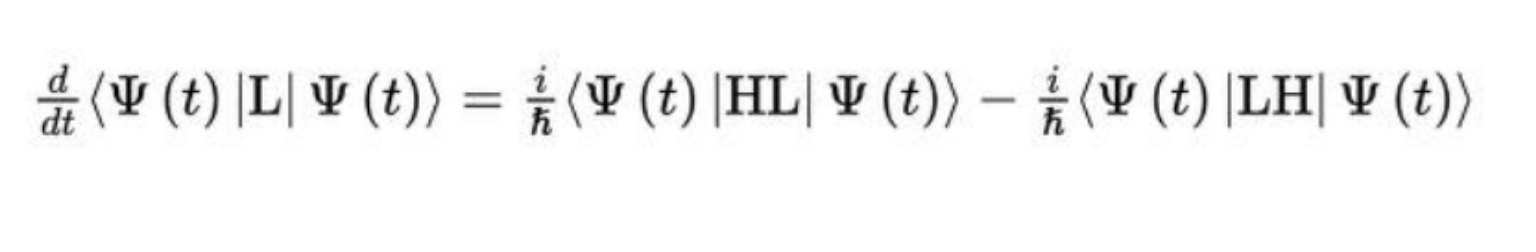
\includegraphics[width=.9\linewidth]{2022-03-04_09-28-18_screenshot.png}
\end{center}

back.

We can summarize this expression to say:

\begin{equation}
   \frac{d}{dt} \big<L\big> = \frac{i}{\hbar} \big<[H, L]\big>
\end{equation}

where, the "commutator" \([A,B] = AB-BA\). (There is a cool property, if you think about it, that \([cA,B] = c[A,B]\).

"the change in expected value by some linear operator \(L\) is that for the commutator \(HL\)". For every observable, its rate of change is proportional to the comutator.

Furthermore, we have some:

\begin{equation}
    [Q,H] = 0
\end{equation}

if observation and evolution has no ordering difference, the change in expected value would be zero.

We can actually decompose \(|\Psi(t)\big>\) down into the sum of all components multiplied to the eigen 

\begin{center}
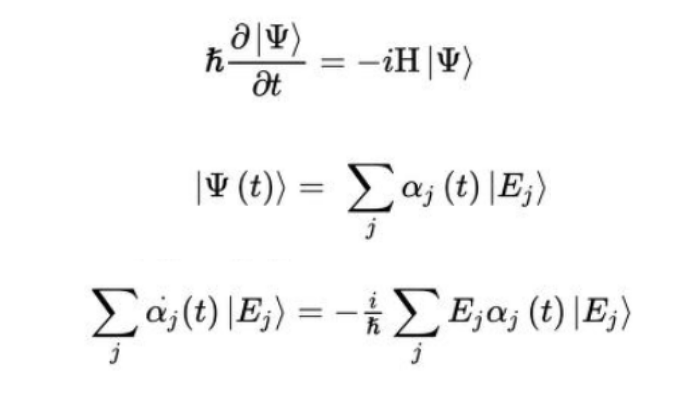
\includegraphics[width=.9\linewidth]{2022-03-04_09-56-38_screenshot.png}
\end{center}


\section{Boolean Operators, etc.}
\label{sec:orgfe02e95}

\subsection{Boolean Inner Product}
\label{sec:org4886948}
Boolean strings of length \(m\), \(x \cdot y\) is their \textbf{\textbf{boolean inner product}}, defined to be:

\begin{equation}
x_1 y_1 \oplus \cdots \oplus x_my_m
\end{equation}

here, \(\oplus\) means exclusive or (addition mod 2) (1+1 is zero, 0+1 is 1, etc.). Odd number of trues is true, even number of trues is false.

\subsection{And now, a boolean network}
\label{sec:orgc041ce2}
We can have a boolean network in classical framing:

\begin{center}
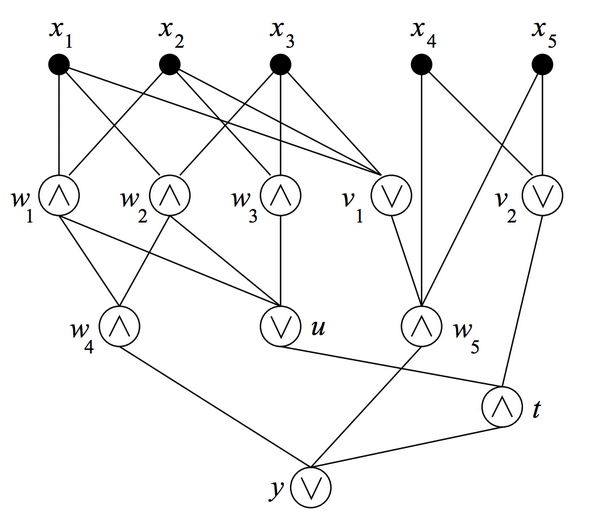
\includegraphics[width=.9\linewidth]{2022-03-02_09-10-04_screenshot.png}
\end{center}

But now, can you simplify this? Is there a simpler way to represent majority---how does the simplest way of computing the majority scale with the inputs.

Does the number of nodes grow proportionally to the number of inputs? I.e.:

\begin{equation}
   \theta(N) =^? \#\ of\ nodes 
\end{equation}

\subsection{Controlled Not}
\label{sec:org903a9c5}
\begin{equation}
   C_{not}(x_1, x_2) = \begin{cases}
x_1\ if\ x_2 = 0\\
1-x_1\ if\ x_2 = 1\\
\end{cases}
\end{equation}


\section{Parallel vs Series}
\label{sec:org99d3168}
\begin{itemize}
\item Tensoring matricies are  parallel operations
\item Producting matricies are series operations
\end{itemize}

\section{Not the Uncertainty Principle}
\label{sec:orgc42eeff}
\begin{itemize}
\item Quantum mechanics is a deterministic theory, but the state lives on the Bloch sphere so has an imaginary component that's not imaginable
\item It propergates counterfactuals
\end{itemize}

The evolution of the state

\section{The Actual Uncertainty Principle}
\label{sec:org2dd8ad9}
Let's take two operators \(\vec{L}\) and \(\vec{M}\). Perhaps one measuring spin in \(\hat{z}\) and one at \(\hat{y}\).

If I was to apply \(L\) to \(|\psi\big>\):

\begin{equation}
   L|\psi\big> = \lambda |\psi \big> 
\end{equation}

We know, that we will get back an eigenvector of \(L\). If you try to observe the answer, you \textbf{will} get an eigenvalue \(\lambda_i\), and \(|\psi\big> \to |\lambda_i\big>\); this takes place with probability of \(\big<\lambda_i|\psi\big>\big<\psi|\lambda_i\big>\).

Because\ldots{}. voodoo witchcraft.

If, for the sake of argument \(\vec{L}\) and \(\vec{M}\) \emph{share} an eigenvector \(|\lambda_i\big>\):

\begin{equation}
   \begin{cases}
L|\lambda_i, \mu_a \big> = \lambda_i | \lambda_i, \mu_a\big>\\
L|\lambda_i, \mu_a \big> = \mu_a | \lambda_i, \mu_a\big>
\end{cases}
\end{equation}

in which, \(|\lambda_i,\mu_a\big>\) is a shared eigenvector between the two operators.

By some trivial commutativity maths, we can get that:

\begin{equation}
   [L, M]\ | \lambda, \mu \big> = 0
\end{equation}

If two operators \(L\), \(M\) share a \emph{complete set of basis} of the eignespace between the two of them, we can plug that into the top expression to figure that \(\forall\ A \in L \cup M\), there is an linear combination of shared eigenvalues \(|\lambda, \mu\big>_i\) which forms \(A\) for every element in both maps. And therefore, if that's true:

\begin{equation}
   [L,M] = 0 
\end{equation}

"\(L\) and \(M\) is commutative".

Hence, IFF two operators share a complete set of eigenvalues do they commute ("application order does not matter").

\noindent\rule{\textwidth}{0.5pt}

Any two Hermitian matrix \(L\) can be written as:

\begin{equation}
   \vec{L} = a \sigma_x  + b \sigma_y+ c \sigma_z+ d I,\ where\ a,b,c,d\in \mathbb{R}^1
\end{equation}

We can figure the result of computating pairwise of these:

\begin{itemize}
\item \([\sigma_x, \sigma_y] = 2i\sigma_z\)
\item \([\sigma_y, \sigma_z] = 2i\sigma_x\)
\item \([\sigma_z, \sigma_x] = 2i\sigma_y\)
\end{itemize}

We can see that the testing in various directions are not commutating (their comutator is not 0).

If two states don't commute (i.e. they don't have shared eigenbases), there \textbf{will} be uncertainty between their measurements. If they do commute, measuring one grantees the measurement of the other.

\noindent\rule{\textwidth}{0.5pt}

The expected value of the operator would be:

\begin{equation}
   \bar{A} = A- \big<A\big> I 
\end{equation}

where, \(\big<A\big> = \big<\psi|A|\psi\big> = \sum_a aP(a)\) for any some \(\psi\).

"the expected value of the state is simply an eigenvalue measuring the state times the probability of it coming up (remember that all results of \(A|\psi\big>\) are eigenvectors of \(A\)).

Recall also from statistics:

\begin{equation}
   (\Delta A)^2 = \sum_a  (a- \big<A\big>)^2 P(a) 
\end{equation}

And finally, this would be equal to (given the same principle above) the expected value of \((\Delta A)^2\).

After much skipped linear algebra, we motivate finally to one more result: 

\begin{equation}
   \Delta A \Delta B \leq \frac{1}{2} |\big<\psi|[A,B] |\psi\big>|
\end{equation}

The expected value of the commutator is twice the variance in both \(A\) and \(B\) if they don't commute. "The uncertainty cannot be lower than of the commutator."

If the comutator is zero, then, it is possible for the uncertainties of the operators to be zero; otherwise the uncertainties in the operator \emph{must be} nonzero.

Cool result: for instance, if you recall \([\sigma_x, \sigma_y] = 2 i\sigma_z\). If you keep testing towards the \(x\) and \(y\) directions, you will expect it to eventually converge to the \(z\) direction per the statement above.

\section{Basically Feasible Operations}
\label{sec:org3b07d05}
The Hadamand matrix \(H_N\) of order \(N\) is defined:

\begin{equation}
    H_2 = H, \forall N \geq 4
\end{equation}

It is defined as such:

\begin{equation}
   H_N = H_{N/2} \otimes H = \frac{1}{\sqrt{2}} \begin{bmatrix}
H_{N/2} & H_{N/2} \\
H_{N/2} & -H_{N/2} 
\end{bmatrix}
\end{equation}

We can also define \(H_N\) as:

\begin{equation}
   H_N[r, c] = (-1)^{r \cdot c} 
\end{equation}

where \(r \cdot c\) is the inner product of \(r\) and \(c\) are boolean strings.

\(N = 2^n\), \(N\) is the number of states, \(N\) is the number of cubits.

\subsection{Fourier Matrix}
\label{sec:org5a131ce}
Some other application, the Fourier matrix:

Let \(\omega\) stand for \(e^{2\pi i / N}\), which is considered "the" principal \(N\) root of unity. The Fourier matrix \(F_N\) of order \(N\) is defined as:

\begin{equation}
   F_N [i,j] = \omega^{ij\ mod\ N} 
\end{equation}

We take the mod-n between \(i\) and \(j\). 

"we take something hugely complicated, put in in a huge space, and make it linear."

\subsection{Toffoli Gate}
\label{sec:orga4dc38a}
Define the Tofoli gate as the ternary Boolean function

\begin{equation}
   TOF(x_1, x_2, x_3) = (x_1, x_2, x_3 \oplus (x_1 \wedge x_3)) 
\end{equation}

This is very useful:

\begin{itemize}
\item \(NOT(a) = TOF(1,1,a)\)
\item \(AND(a,b) = TOF(a,b,0)\)
\item \(OR(a,b) = NOT(AND(NOT(a), NOT(b)))\)
\end{itemize}

And tada we have all of logic.

The toffoli gate can be represented as a \(8\) by \(8\) matrix, with only the last smallest quadrant flipped:

\begin{equation}
   \begin{pmatrix}
1 & 0 & 0 &0 &0&0&0&0 \\
0 & 1 & 0 &0 &0&0&0&0 \\
0 & 0 & 1 &0 &0&0&0&0 \\
0 & 0 & 0 &1 &0&0&0&0 \\
0 & 0 & 0 &0 &1&0&0&0 \\
0 & 0 & 0 &0 &0&1&0&0 \\
0 & 0 & 0 &0 &0&0&0&1 \\
0 & 0 & 0 &0 &0&0&1&0 \\
\end{pmatrix} 
\end{equation}

You can see that, unless the last values are true, nothing happens (its mostly the identity.) However, if the last group is true, we will flip the last value.
\end{document}